% Provenance (never printed): see sources/outline_sources.md (Year 3:
% sequence stratigraphy, accommodation and supply, systems tracts,
% cyclostratigraphy). Brief: sources/book5/BRIEFS.md, ch. 16. Curves from
% figdata/bachelor-3/shelf_model.py and lr04_periodogram.py. Exercise and
% problem values in the Book 5 scratch calculator calc/ch16.py. The Varden
% basin, its shelf and its core are invented.
\chapter{Estratigrafía secuencial}\label{ch:b3:sequence-stratigraphy}

A lo largo de una sección sísmica de un margen continental, los reflectores se apoyan sobre los más antiguos,
luego avanzan hacia la cuenca, después retroceden hacia tierra firme, y
el patrón se repite más arriba. Cada paquete registra una pugna entre
dos tasas: la tasa a la que se crea espacio para el sedimento, por subsidencia y por
el ascenso del mar, y la tasa a la que los ríos lo rellenan. La estratigrafía
secuencial lee la pugna a partir de la geometría de las capas, y
la \omterm{def:b3:sequence-stratigraphy:cyclo}{cicloestratigrafía} lee su reloj a partir de su espesor.

\begin{recall}
El espacio de acomodación, la eustasia, el nivel relativo del mar, la subsidencia y la
cuenca sedimentaria están en el volumen de primer año, en su capítulo sobre diagénesis y
cuencas sedimentarias. La transgresión y la regresión marinas y el ciclo de nivel del mar
de primer orden están en el volumen de segundo año, en su capítulo sobre la Tierra fanerozoica; los
parámetros de Milankovitch y la precesión climática en su capítulo sobre forzamiento orbital
y las edades glaciales; el modelo de edad en su capítulo sobre archivos climáticos
y proxies. \omterm{def:b3:exploration-seismology:terminations}{Onlap}, \omterm{def:b3:exploration-seismology:terminations}{downlap}, \omterm{def:b3:exploration-seismology:terminations}{toplap}, \omterm{def:b3:exploration-seismology:terminations}{truncación erosiva} y \omterm{def:b3:exploration-seismology:seismic-stratigraphy}{estratigrafía
sísmica} se tratan en el capítulo~\ref{ch:b3:exploration-seismology}. Las series de Fourier
y la transformada de Fourier están en los libros de matemáticas.
\end{recall}

\section{Acomodación, aporte sedimentario y línea de costa}\label{sec:b3:sequence-stratigraphy:shoreline}

En cualquier punto de una cuenca el nivel relativo del mar sube a la tasa $A = \dot E
+ \sigma$, la tasa eustática más la de subsidencia (un descenso cuando $A < 0$).
El nivel relativo del mar en un lugar viene fijado por el nivel global del mar y por
todo lo que mueve el terreno que hay debajo: la \omterm{def:b3:lithosphere-thermal-models:thermal-subsidence}{subsidencia térmica}, la carga del
sedimento y la flexión que provoca, el rebote de la corteza tras el
deshielo de un casquete de hielo, y el lento empuje del manto bajo la placa.
El ascenso del nivel relativo del mar crea espacio de acomodación; el sedimento lo rellena. Que la
línea de costa avance hacia el mar o hacia tierra depende de ambos, y no del nivel del mar
por sí solo.
% ledger: miller20:rsl

\begin{definition}[Regresión normal y forzada]\label{def:b3:sequence-stratigraphy:regression}
Una \emph{regresión normal}\index{regresión normal} es un avance hacia el mar de la
línea de costa mientras el nivel relativo del mar sube: el aporte supera al
espacio de acomodación generado en la costa. Una \emph{regresión forzada}\index{regresión forzada}
es un avance hacia el mar impulsado por un descenso del nivel relativo del mar: la
línea de costa es empujada hacia la cuenca sea cual sea el aporte, y el terreno que queda
atrás queda expuesto y erosionado.
\end{definition}

\begin{definition}[Trayectoria de la línea de costa]\label{def:b3:sequence-stratigraphy:trajectory}
La \emph{trayectoria de la línea de costa}\index{trayectoria de la línea de costa} es el camino de
la línea de costa a lo largo del tiempo, dibujada en una sección de buzamiento, en el marco de referencia del
sedimento, de modo que muestra tanto el desplazamiento horizontal de la línea de costa como su
ascenso o descenso relativo a las capas inferiores.
\end{definition}

Un perfil sencillo hace exacta la pugna. Tras la línea de costa, una plataforma superior plana
de anchura $W$ se encuentra al nivel del mar; frente a ella, un talud frontal de pendiente
$\tan\theta$ desciende hasta el fondo de la cuenca, a una altura $D$ por debajo. El aporte
sedimentario $Q$ es un volumen por unidad de tiempo y por metro de costa (un área por
unidad de tiempo en la sección).

\begin{proposition}[Trayectoria de la línea de costa]\label{prop:b3:sequence-stratigraphy:trajectory}
Si el nivel relativo del mar sube ($A \ge 0$) y la plataforma superior se recrece
uniformemente, la línea de costa se desplaza a
\[
\frac{\mathrm dx_s}{\mathrm dt} = \frac{Q - AW}{D};
\]
prograda mientras $Q > AW$ y retrocede cuando $AW > Q$. Si el nivel relativo del mar
desciende ($A < 0$), la plataforma superior no recibe nada y
\[
\frac{\mathrm dx_s}{\mathrm dt} = \frac{Q}{D} + \frac{|A|}{\tan\theta}.
\]
En ambos casos la trayectoria asciende o desciende con el ángulo cuya tangente es
$A/(\mathrm dx_s/\mathrm dt)$.
\end{proposition}

\begin{proof}
En un tiempo $\mathrm dt$ la plataforma superior necesita $AW\,\mathrm dt$ de sedimento para
mantenerse al nivel del mar. Lo que sobra, $(Q - AW)\,\mathrm dt$, se extiende sobre el talud frontal,
un muro de altura $D$, que avanza $(Q - AW)\,\mathrm dt/D$; un resto negativo
significa que el mar inunda la plataforma superior más deprisa de lo que se rellena. Cuando el mar
desciende, la plataforma superior queda sobre el agua y no recibe nada, y la línea de costa
desciende por el antiguo talud frontal $|A|\,\mathrm dt/\tan\theta$ sin ningún
sedimento, mientras que todo el aporte construye el talud hacia delante por $Q\,\mathrm
dt/D$. La línea de costa sube $A\,\mathrm dt$ respecto a las capas inferiores
mientras avanza $\mathrm dx_s$, lo que da el ángulo.
\end{proof}

Una \omterm{def:b3:sequence-stratigraphy:regression}{regresión normal} necesita, por tanto, un aporte mayor que el espacio de acomodación
generado en la plataforma superior, y su trayectoria asciende; una \omterm{def:b3:sequence-stratigraphy:regression}{regresión forzada} se produce
sea cual sea el aporte, y su trayectoria desciende. La razón entre las dos tasas,
a menudo escrita $A/S$, clasifica los patrones: progradación cuando $A/S < 1$ en la
plataforma superior, agradación cerca de 1, retrogradación por encima. La misma curva del nivel del mar
puede dar, por tanto, una regresión en un margen rico en sedimento y una
transgresión en uno pobre en sedimento.

\section{Geometría estratal: secuencias y cortejos sedimentarios}\label{sec:b3:sequence-stratigraphy:sequences}

Las terminaciones de reflector del capítulo~\ref{ch:b3:exploration-seismology}
son el vocabulario del método: \omterm{def:b3:exploration-seismology:terminations}{onlap} y \omterm{def:b3:exploration-seismology:terminations}{downlap} marcan la base de un
paquete, \omterm{def:b3:exploration-seismology:terminations}{toplap} y \omterm{def:b3:exploration-seismology:terminations}{truncación erosiva} su techo. Leídas en una sección de buzamiento,
dividen un margen en paquetes limitados por superficies de no sedimentación o
erosión, y cada uno registra un ciclo del nivel relativo del mar.

\begin{definition}[Secuencia deposicional y límite de secuencia]\label{def:b3:sequence-stratigraphy:sequence}
Una \emph{secuencia deposicional}\index{secuencia deposicional} es una sucesión
de estratos genéticamente relacionados, sin discontinuidades mayores en su interior, limitada en su base
y en su techo por discordancias o por las concordancias que las prolongan hacia la
cuenca. Su superficie limitante es el \emph{límite
de secuencia}\index{límite de secuencia}: una discordancia excavada por exposición y
erosión en la plataforma durante un descenso del nivel relativo del mar, que pasa hacia la cuenca
a una concordancia correlativa.
\end{definition}

\begin{definition}[Cortejo sedimentario]\label{def:b3:sequence-stratigraphy:tract}
Un \emph{cortejo sedimentario}\index{cortejo sedimentario} es el conjunto de sistemas
deposicionales (fluvial, costero, de plataforma, de talud) que estuvieron activos juntos durante una
parte de un ciclo del nivel relativo del mar, reconocido por su posición en la
secuencia, por sus superficies limitantes y su patrón de apilamiento. Se distinguen
cuatro:
\begin{itemize}
\item el \emph{cortejo de nivel descendente}\index{cortejo de nivel descendente},
  construido por \omterm{def:b3:sequence-stratigraphy:regression}{regresión forzada} mientras desciende el nivel relativo del mar:
  foresets en escalón descendente, separados de la antigua plataforma;
\item el \emph{cortejo de nivel bajo}\index{cortejo de nivel bajo},
  construido por \omterm{def:b3:sequence-stratigraphy:regression}{regresión normal} una vez que el nivel relativo del mar vuelve a subir,
  en la posición más baja de la línea de costa: una cuña con agradación y progradación;
\item el \emph{cortejo transgresivo}\index{cortejo transgresivo},
  construido mientras la línea de costa retrocede hacia tierra: unidades retrogradantes
  que hacen \omterm{def:b3:exploration-seismology:terminations}{onlap} sobre la antigua plataforma;
\item el \emph{cortejo de nivel alto}\index{cortejo de nivel alto},
  construido por \omterm{def:b3:sequence-stratigraphy:regression}{regresión normal} al final de la subida, cuando el aporte vuelve a superar
  al espacio de acomodación: foresets que progradan y hacen \omterm{def:b3:exploration-seismology:terminations}{downlap} sobre los depósitos subyacentes.
\end{itemize}
\end{definition}

\begin{definition}[Superficie transgresiva y de máxima inundación]\label{def:b3:sequence-stratigraphy:surfaces}
La \emph{superficie transgresiva}\index{superficie transgresiva} es la primera
\omterm{def:b3:sequence-stratigraphy:parasequence}{superficie de inundación} significativa por encima de los depósitos de nivel bajo: marca el giro
de la línea de costa de la regresión a la transgresión. La \emph{superficie de máxima
inundación}\index{superficie de máxima inundación} marca la posición más hacia tierra de
la línea de costa, el cambio de la transgresión a la regresión de nivel alto; los
foresets de nivel alto hacen \omterm{def:b3:exploration-seismology:terminations}{downlap} sobre ella.
\end{definition}

\begin{definition}[Sección condensada y valle inciso]\label{def:b3:sequence-stratigraphy:condensed}
Una \emph{sección condensada}\index{sección condensada} es un intervalo delgado
depositado muy lentamente lejos de la línea de costa mientras el mar inunda la plataforma
y el sedimento queda retenido cerca de la costa: unos pocos centímetros o decímetros
de arcilla, fósiles, glauconita o fosfato que puede registrar un tiempo largo. Un
\emph{valle inciso}\index{valle inciso} es un valle fluvial excavado en la
plataforma expuesta mientras desciende el nivel relativo del mar, y rellenado durante el
nivel bajo y la transgresión siguientes.
\end{definition}

\begin{omfigure}
\begin{tikzpicture}[font=\scriptsize, x=0.9cm, y=1.25cm, >=Stealth]
% older highstand deposits below the sequence boundary
\fill[black!10] (0,0) -- (14,0) -- (14,0.4) -- (10,0.6) -- (6,2.8) -- (0,3.0) -- cycle;
\draw[black!35] (1.5,2.0) .. controls (3.2,1.95) and (4.5,1.2) .. (8.5,0.45);
\draw[black!35] (3.5,2.93) .. controls (4.8,2.85) and (6,1.6) .. (10.5,0.42);
% falling-stage systems tract
\fill[red!25] (6.0,2.8) -- (7.4,2.25) -- (8.4,1.85) -- (9.4,1.35) -- (10.4,0.75) -- (10.6,0.58) -- (10,0.6) -- cycle;
\draw[red!60!black] (6.6,2.56) .. controls (7.0,2.4) and (7.5,1.95) .. (8.0,1.70);
\draw[red!60!black] (7.6,2.17) .. controls (8.0,2.0) and (8.5,1.45) .. (9.0,1.15);
\draw[red!60!black] (8.6,1.75) .. controls (9.0,1.55) and (9.5,0.9) .. (10.0,0.6);
% lowstand wedge
\fill[orange!40] (9.2,1.45) -- (10.4,1.5) -- (11.5,1.0) -- (12.6,0.6) -- (13.4,0.44) -- (10.6,0.58) -- (10.4,0.75) -- cycle;
% incised valley and its fill
\fill[orange!30] (2.9,2.9) .. controls (3.3,2.3) and (3.9,2.3) .. (4.3,2.86) -- cycle;
% transgressive systems tract
\fill[green!45!black!35] (11.5,1.0) -- (10.4,1.5) -- (9.2,1.45) -- (8.4,1.85) -- (7.4,2.25) -- (6.0,2.8) -- (1.0,2.97) -- (1.0,3.05) -- (6.0,2.95) -- (7.6,2.5) -- (9.4,1.75) -- (10.8,1.45) -- cycle;
% highstand systems tract
\fill[blue!22] (0,3.62) -- (7.5,3.42) -- (9.8,2.2) -- (11.2,1.22) -- (10.8,1.45) -- (9.4,1.75) -- (7.6,2.5) -- (6.0,2.95) -- (1.0,3.05) -- (0,3.07) -- cycle;
\draw[blue!60!black] (4.0,3.52) .. controls (5.0,3.45) and (5.8,3.1) .. (6.6,2.79);
\draw[blue!60!black] (5.6,3.47) .. controls (6.6,3.4) and (7.4,2.8) .. (8.2,2.26);
\draw[blue!60!black] (6.8,3.44) .. controls (7.8,3.35) and (8.8,2.4) .. (9.7,1.69);
% surfaces
\draw[red!70!black, very thick] (0,3.0) -- (2.9,2.9) .. controls (3.3,2.3) and (3.9,2.3) .. (4.3,2.86) -- (6.0,2.8) -- (7.4,2.25) -- (8.4,1.85) -- (9.2,1.45);
\draw[red!70!black, very thick, densely dashed] (9.2,1.45) -- (9.4,1.35) -- (10.4,0.75) -- (10.6,0.58) -- (14,0.4);
\draw[green!40!black, thick] (11.5,1.0) -- (10.4,1.5) -- (9.2,1.45);
\draw[blue!60!black, thick] (0,3.07) -- (1.0,3.05) -- (6.0,2.95) -- (7.6,2.5) -- (9.4,1.75) -- (10.8,1.45) -- (11.5,1.03) -- (12.6,0.63) -- (13.4,0.47) -- (14,0.43);
% labels
\node[blue!50!black] at (2.6,3.36) {nivel alto (HST)};
\node[green!35!black, anchor=south] at (4.8,3.92) {transgresivo (TST)};
\draw[green!35!black] (4.8,3.92) -- (4.4,3.01);
\node[red!60!black, anchor=west] at (10.1,2.45) {nivel descendente (FSST)};
\draw[red!60!black] (10.1,2.45) -- (8.8,1.62);
\node[orange!60!black, anchor=west] at (12.2,1.55) {nivel bajo (LST)};
\draw[orange!60!black] (12.2,1.55) -- (11.2,0.85);
\node[anchor=north, align=center] at (3.6,2.25) {valle\\ inciso};
\node[red!70!black, anchor=north] at (1.4,2.95) {SB};
\node[red!70!black, anchor=north] at (12.0,0.38) {concordancia correlativa};
\node[blue!60!black, anchor=west] at (12.7,1.1) {MFS};
\draw[blue!60!black] (12.7,1.1) -- (12.1,0.82);
\node[green!40!black, anchor=west] at (11.6,2.0) {TS};
\draw[green!40!black] (11.6,2.0) -- (10.9,1.27);
\node[blue!60!black, anchor=south] at (13.4,0.58) {condensada};
\node[anchor=west, black!60] at (0.2,0.35) {depósitos antiguos};
\draw[->] (11.2,3.9) -- (12.6,3.9) node[right] {hacia la cuenca};
\end{tikzpicture}

\par\smallskip{\small Anatomía de una \omterm{def:b3:sequence-stratigraphy:sequence}{secuencia deposicional} en una sección paralela al buzamiento
(esquemática, con la escala vertical muy exagerada). El \omterm{def:b3:sequence-stratigraphy:sequence}{límite de secuencia} (SB, por sus siglas en inglés, en rojo)
es una discordancia en la plataforma, con un \omterm{def:b3:sequence-stratigraphy:condensed}{valle inciso}, y una
concordancia correlativa en la cuenca (a trazos); aquí se dibuja por encima de los
depósitos de nivel descendente. La \omterm{def:b3:sequence-stratigraphy:surfaces}{superficie transgresiva} (TS, por sus siglas en inglés) corona la cuña de nivel bajo; la \omterm{def:b3:sequence-stratigraphy:surfaces}{superficie de
máxima inundación} (MFS, por sus siglas en inglés) corona el delgado \omterm{def:b3:sequence-stratigraphy:tract}{cortejo transgresivo} y pasa hacia la cuenca
a una \omterm{def:b3:sequence-stratigraphy:condensed}{sección condensada}; los foresets de nivel alto hacen \omterm{def:b3:exploration-seismology:terminations}{downlap} sobre ella.}\label{fig:b3:sequence-stratigraphy:anatomy}
\end{omfigure}

Dónde discurre exactamente el \omterm{def:b3:sequence-stratigraphy:sequence}{límite de secuencia} en la cuenca es una convención, y
los autores no coinciden: algunos lo trazan en la base de los depósitos de nivel descendente, donde
el descenso comienza, otros en su techo, donde termina, como en la figura anterior.
En la plataforma no hay ambigüedad: el límite es la superficie de exposición
y erosión, y los depósitos situados encima son más jóvenes que el descenso.

Leída de abajo arriba en un punto de la plataforma externa, una secuencia registra
el ciclo: foresets de nivel alto, una superficie de exposición, quizá un relleno de valle,
la \omterm{def:b3:sequence-stratigraphy:surfaces}{superficie transgresiva}, capas retrogradantes, un intervalo condensado en la
\omterm{def:b3:sequence-stratigraphy:surfaces}{superficie de máxima inundación}, y luego de nuevo foresets de nivel alto. La jerarquía de los
ciclos la fijan sus causas: la apertura y el cierre de los océanos para el
ciclo de primer orden, los cambios en el volumen de hielo y en la velocidad de
expansión del fondo oceánico para los más cortos, y la tectónica local y el aporte para todos
ellos.

\section{Parasecuencias y patrones de apilamiento}\label{sec:b3:sequence-stratigraphy:parasequences}

Dentro de un \omterm{def:b3:sequence-stratigraphy:tract}{cortejo sedimentario}, los paquetes más pequeños que un geólogo cartografía en un acantilado o en un registro de pozo
son unidades de somerización hacia arriba de entre unos pocos metros y algunas decenas de metros de espesor,
coronadas por una superficie donde el agua profunda vuelve bruscamente.

\begin{definition}[Parasecuencia y superficie de inundación]\label{def:b3:sequence-stratigraphy:parasequence}
Una \emph{parasecuencia}\index{parasecuencia} es una sucesión relativamente concordante
de capas de origen genético relacionado, limitada por superficies de inundación, en la que
el agua se hace más somera hacia arriba: en una costa dominada por el oleaje, el lodo de mar adentro pasa hacia arriba
a arena de anteplaya inferior y superior, y a playa. Una \emph{superficie de
inundación}\index{superficie de inundación} es una superficie a través de la cual facies de agua más profunda se superponen bruscamente a otras más someras,
con indicios de una profundización súbita.
\end{definition}

Una \omterm{def:b3:sequence-stratigraphy:parasequence}{parasecuencia} aislada se vuelve más gruesa hacia arriba, y su registro de rayos gamma, bajo en arena
y alto en arcilla, dibuja una forma de embudo que se estrecha hacia arriba. La forma en que se apilan las
\omterm{def:b3:sequence-stratigraphy:parasequence}{parasecuencias} de un cortejo indica la tendencia de la línea de costa:
cada una se construyó más mar adentro que la anterior (progradante),
encima de la anterior (agradante) o hacia tierra respecto a ella (retrogradante). Un registro
a través del apilamiento muestra la tendencia directamente: cada \omterm{def:b3:sequence-stratigraphy:parasequence}{parasecuencia} termina en
facies más gruesas y más someras que la de debajo, iguales, o más finas y más profundas.
Los \omterm{def:b3:sequence-stratigraphy:tract}{cortejos de nivel alto} y de nivel bajo se apilan de forma progradante o agradante,
los transgresivos, de forma retrogradante. El capítulo siguiente lee estos registros
facies por facies.

\begin{omfigure}
\begin{tikzpicture}[font=\scriptsize, x=1cm, y=1cm]
% three logs: each parasequence a coarsening-upward wedge (grain size to the right)
% progradational
\begin{scope}[xshift=0cm]
\fill[yellow!45!brown!35] (0,0) -- (0.5,0) -- (1.4,1.1) -- (0,1.1) -- cycle;
\fill[yellow!45!brown!35] (0,1.1) -- (0.5,1.1) -- (1.8,2.2) -- (0,2.2) -- cycle;
\fill[yellow!45!brown!35] (0,2.2) -- (0.5,2.2) -- (2.2,3.3) -- (0,3.3) -- cycle;
\draw (0,0) -- (0.5,0) -- (1.4,1.1) -- (0.5,1.1) -- (1.8,2.2) -- (0.5,2.2) -- (2.2,3.3) -- (0,3.3) -- cycle;
\node[anchor=north, align=center] at (1.1,-0.1) {progradacional\\ (la línea de costa avanza hacia el mar)};
\end{scope}
% aggradational
\begin{scope}[xshift=4.2cm]
\fill[yellow!45!brown!35] (0,0) -- (0.5,0) -- (1.8,1.1) -- (0,1.1) -- cycle;
\fill[yellow!45!brown!35] (0,1.1) -- (0.5,1.1) -- (1.8,2.2) -- (0,2.2) -- cycle;
\fill[yellow!45!brown!35] (0,2.2) -- (0.5,2.2) -- (1.8,3.3) -- (0,3.3) -- cycle;
\draw (0,0) -- (0.5,0) -- (1.8,1.1) -- (0.5,1.1) -- (1.8,2.2) -- (0.5,2.2) -- (1.8,3.3) -- (0,3.3) -- cycle;
\node[anchor=north, align=center] at (1.1,-0.1) {agradacional\\ (la línea de costa se mantiene)};
\end{scope}
% retrogradational
\begin{scope}[xshift=8.4cm]
\fill[yellow!45!brown!35] (0,0) -- (0.5,0) -- (2.2,1.1) -- (0,1.1) -- cycle;
\fill[yellow!45!brown!35] (0,1.1) -- (0.5,1.1) -- (1.8,2.2) -- (0,2.2) -- cycle;
\fill[yellow!45!brown!35] (0,2.2) -- (0.5,2.2) -- (1.4,3.3) -- (0,3.3) -- cycle;
\draw (0,0) -- (0.5,0) -- (2.2,1.1) -- (0.5,1.1) -- (1.8,2.2) -- (0.5,2.2) -- (1.4,3.3) -- (0,3.3) -- cycle;
\node[anchor=north, align=center] at (1.1,-0.1) {retrogradacional\\ (la línea de costa retrocede hacia tierra)};
\end{scope}
% flooding surfaces
\foreach \s in {0,4.2,8.4} {
  \draw[omDef, thick] (\s-0.15,1.1) -- (\s+2.5,1.1);
  \draw[omDef, thick] (\s-0.15,2.2) -- (\s+2.5,2.2);
  \node[omDef, anchor=west] at (\s+2.5,1.1) {FS};
  \node[omDef, anchor=west] at (\s+2.5,2.2) {FS};
}
% grain-size axis
\draw[->] (0,3.6) -- (2.3,3.6) node[right] {más grueso};
\node[anchor=east] at (0,3.6) {lodo};
\end{tikzpicture}

\par\smallskip{\small Tres \omterm{def:b3:sequence-stratigraphy:parasequence}{parasecuencias} apiladas de tres maneras, dibujadas como
registros de tamaño de grano (la anchura hacia la derecha indica mayor tamaño de grano). Cada \omterm{def:b3:sequence-stratigraphy:parasequence}{parasecuencia}
se engrosa hacia arriba desde lodo de mar adentro hasta arena de anteplaya, y termina en una
\omterm{def:b3:sequence-stratigraphy:parasequence}{superficie de inundación} (FS); la parte superior de cada una es más gruesa que la de debajo cuando el
apilamiento es progradante, igual cuando es agradante, más fina cuando
es retrogradante.}\label{fig:b3:sequence-stratigraphy:stacking}
\end{omfigure}

\begin{inthefield}[Parasecuencias en un acantilado desértico]
\begin{minipage}[t]{0.52\linewidth}\vspace{0pt}
Los Book Cliffs del este de Utah exponen depósitos de línea de costa del Cretácico superior
a lo largo de decenas de kilómetros. En el Miembro Kenilworth, seguido a lo largo de los acantilados
desde Price hasta Hatch Mesa, los geólogos cartografiaron depósitos de llanura costera, de anteplaya,
de plataforma interna y de \omterm{def:b3:sequence-stratigraphy:condensed}{valle inciso}, y nueve \omterm{def:b3:sequence-stratigraphy:parasequence}{parasecuencias} de engrosamiento hacia arriba,
dominadas por el oleaje o por tormentas, de 7 a \qty{32}{m} de espesor. Hacia la cuenca cada una
se divide en hasta cuatro conjuntos de capas más pequeños, de engrosamiento hacia arriba, de 2 a
\qty{18}{m} de espesor; algunas arenas de anteplaya descansan sobre una base neta, que el
estudio interpreta como depósitos de nivel bajo.
\end{minipage}\hfill
\begin{minipage}[t]{0.44\linewidth}\vspace{0pt}
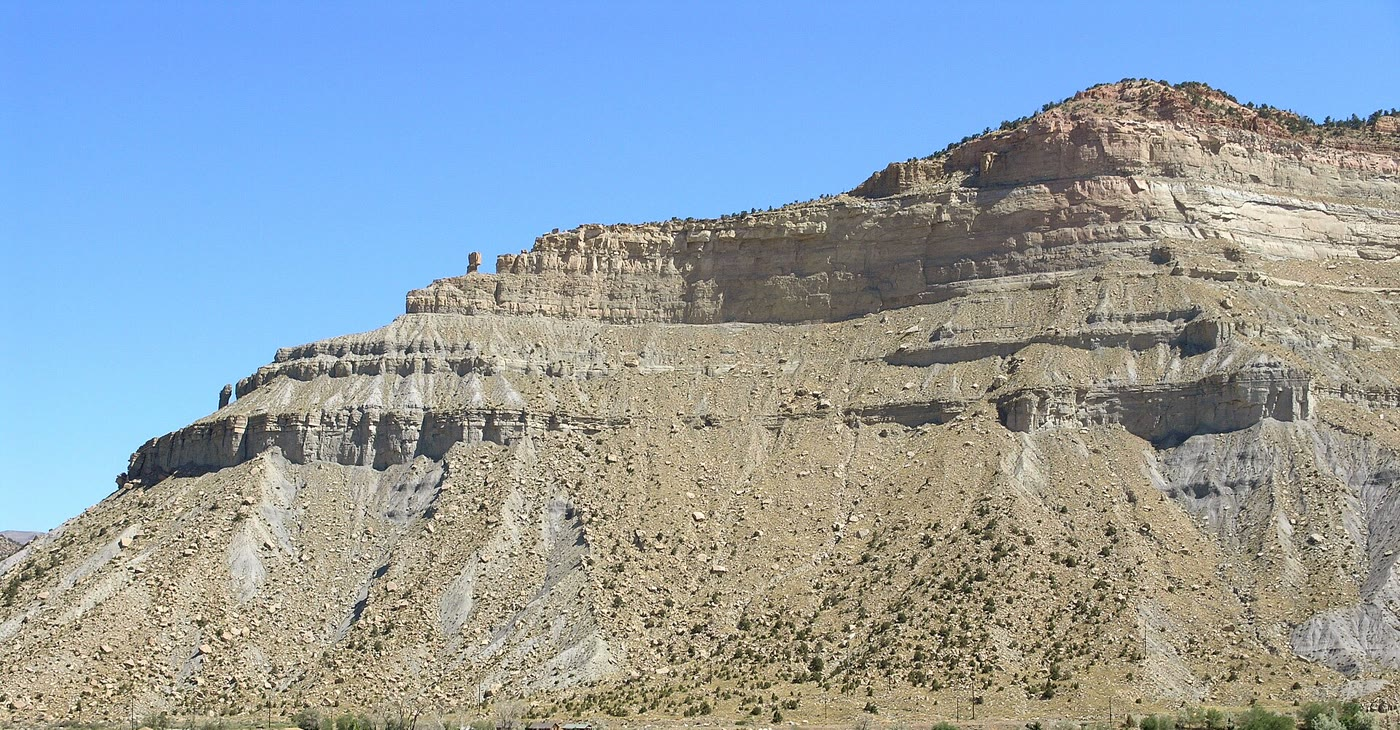
\includegraphics[width=\linewidth]{images/book5/b3-book-cliffs-helper.jpg}

{\scriptsize Los Book Cliffs sobre Helper, Utah: repisas de arenisca pálida destacan
por encima de laderas de lodolita gris. Fotografía de David Mackie, dominio público.}
\end{minipage}
\end{inthefield}
% ledger: pattison95:kenilworth, photo:b3-book-cliffs

\section{Un modelo directo de una plataforma}\label{sec:b3:sequence-stratigraphy:model}

Las reglas de las secciones anteriores pueden ejecutarse como un modelo. La cuenca de Varden
es una plataforma inventada: una rampa con pendiente hacia la cuenca de \qty{1.5}{m/km}, con subsidencia
de $\sigma = 0.02 + x/1200$ \unit{m/kyr} a una distancia $x$ (km) de la
charnela, bajo un nivel del mar $E = -30\cos(2\pi t/400)$ (m, $t$ en kyr), alimentado por un
río que aporta $Q = \qty{6000}{m^3/kyr}$ por metro de costa. En cada paso
de medio millar de años la cuenca se hunde; el sedimento rellena entonces un topset plano
hasta el nivel del mar, donde la superficie antigua está bajo el agua, y un
foreset de pendiente 0.012 frente a él, situando la línea de costa de modo que el
volumen añadido iguale al aporte; el terreno emergido no recibe nada y, por
simplicidad, no se erosiona. El modelo parte de un nivel bajo del mar, tras una primera
cuña construida con nivel del mar constante.

\begin{omfigure}
\begin{tikzpicture}
\begin{groupplot}[group style={group size=1 by 2, vertical sep=0.35cm, x descriptions at=edge bottom},
  omrecord, width=0.86\linewidth, xmin=0, xmax=600,
  xtick={0,100,200,300,400,500,600},
  tick label style={font=\scriptsize}, label style={font=\small}]
\nextgroupplot[height=0.2\linewidth, ylabel={$E$ (m)}, ymin=-35, ymax=35,
  ytick={-30,0,30}]
\addplot[omDef, thick, domain=0:600, samples=121] {-30*cos(deg(2*pi*x/400))};
\nextgroupplot[height=0.3\linewidth, xlabel={tiempo (kyr)}, ylabel={línea de costa $x_s$ (km)},
  ymin=0, ymax=60, ytick={0,20,40,60},
  scatter/classes={1={mark=*, red!70!black}, 2={mark=*, orange!80!black},
    3={mark=*, green!50!black}, 4={mark=*, blue!70!black}}]
% computed in figdata/bachelor-3/shelf_model.py
\addplot[scatter, only marks, mark size=0.9pt, scatter src=explicit symbolic]
  table[x=t, y=xs, meta=tract] {figdata/out/bachelor-3-shelf_model-shore.dat};
\node[font=\scriptsize, orange!60!black] at (axis cs:12,56) {LST};
\node[font=\scriptsize, green!40!black] at (axis cs:70,40) {TST};
\node[font=\scriptsize, blue!60!black] at (axis cs:160,6) {HST};
\node[font=\scriptsize, red!60!black] at (axis cs:300,22) {FSST};
\node[font=\scriptsize, orange!60!black] at (axis cs:415,57) {LST};
\node[font=\scriptsize, green!40!black] at (axis cs:520,45) {TST};
\node[font=\scriptsize, blue!60!black] at (axis cs:580,12) {HST};
\end{groupplot}
\end{tikzpicture}

\par\smallskip{\small Arriba, el nivel eustático del mar del modelo de Varden;
abajo, la posición de la línea de costa, coloreada según el \omterm{def:b3:sequence-stratigraphy:tract}{cortejo sedimentario} (nivel bajo
naranja, transgresivo verde, nivel alto azul, nivel descendente rojo), clasificada
únicamente a partir de los resultados del modelo: nivel descendente mientras el nivel relativo del mar desciende
en la línea de costa, transgresivo mientras la línea de costa retrocede, nivel bajo o
nivel alto mientras avanza bajo un mar en ascenso, tras un descenso o tras una
transgresión.}\label{fig:b3:sequence-stratigraphy:series}
\end{omfigure}

La figura superior sigue la línea de costa a lo largo del tiempo, y la inferior
muestra los depósitos que dejó. Los cortejos aparecen sin ninguna regla escrita en el
modelo más allá del relleno y la subsidencia. La cuña de nivel bajo del inicio se sitúa muy
mar adentro; el mar en ascenso desplaza la línea de costa \qty{38}{km} hacia tierra en la primera
transgresión, y los foresets de nivel alto vuelven a progradar a medida que el ascenso se ralentiza.
Luego comienza el descenso: la línea de costa es empujada hacia la cuenca \qty{33}{km} en
\qty{187}{kyr}, dejando foresets delgados en escalón descendente y una plataforma emergida
detrás, el \omterm{def:b3:sequence-stratigraphy:tract}{cortejo de nivel descendente}. Siguen una nueva cuña de nivel bajo, una segunda transgresión
y un nuevo nivel alto. La velocidad de la \omterm{def:b3:sequence-stratigraphy:regression}{regresión forzada} en el modelo
concuerda con la fórmula de la proposición con un margen de unos pocos por ciento; bajo un
mar en ascenso el topset del modelo no sufre agradación uniforme, ya que la subsidencia
crece hacia la cuenca, y la fórmula es solo una guía.

\begin{omfigure}
\begin{tikzpicture}
\begin{axis}[omsection, width=0.95\linewidth, height=0.42\linewidth,
  xmin=0, xmax=70, ymin=-150, ymax=40, clip=true,
  xlabel={distancia hacia la cuenca (km)}, ylabel={elevación actual (m)},
  xtick={0,10,20,30,40,50,60,70}, ytick={-150,-100,-50,0},
  tick label style={font=\scriptsize}, label style={font=\small}]
% computed in figdata/bachelor-3/shelf_model.py
\addplot[fill=black!10, draw=none] table[x=x, y=z0] {figdata/out/bachelor-3-shelf_model-surfaces.dat} -- (axis cs:120,-300) -- (axis cs:0,-300) -- cycle;
\addplot[fill=orange!45, draw=none] table[x=x, y=z] {figdata/out/bachelor-3-shelf_model-poly1.dat};
\addplot[fill=green!45!black!35, draw=none] table[x=x, y=z] {figdata/out/bachelor-3-shelf_model-poly2.dat};
\addplot[fill=blue!25, draw=none] table[x=x, y=z] {figdata/out/bachelor-3-shelf_model-poly3.dat};
\addplot[fill=red!30, draw=none] table[x=x, y=z] {figdata/out/bachelor-3-shelf_model-poly4.dat};
\addplot[fill=orange!45, draw=none] table[x=x, y=z] {figdata/out/bachelor-3-shelf_model-poly5.dat};
\addplot[fill=green!45!black!35, draw=none] table[x=x, y=z] {figdata/out/bachelor-3-shelf_model-poly6.dat};
\addplot[fill=blue!25, draw=none] table[x=x, y=z] {figdata/out/bachelor-3-shelf_model-poly7.dat};
\addplot[black!45, very thin] table[x=x, y=z40] {figdata/out/bachelor-3-shelf_model-surfaces.dat};
\addplot[black!45, very thin] table[x=x, y=z80] {figdata/out/bachelor-3-shelf_model-surfaces.dat};
\addplot[black!45, very thin] table[x=x, y=z120] {figdata/out/bachelor-3-shelf_model-surfaces.dat};
\addplot[black!45, very thin] table[x=x, y=z160] {figdata/out/bachelor-3-shelf_model-surfaces.dat};
\addplot[black!45, very thin] table[x=x, y=z240] {figdata/out/bachelor-3-shelf_model-surfaces.dat};
\addplot[black!45, very thin] table[x=x, y=z280] {figdata/out/bachelor-3-shelf_model-surfaces.dat};
\addplot[black!45, very thin] table[x=x, y=z320] {figdata/out/bachelor-3-shelf_model-surfaces.dat};
\addplot[black!45, very thin] table[x=x, y=z360] {figdata/out/bachelor-3-shelf_model-surfaces.dat};
\addplot[black!45, very thin] table[x=x, y=z440] {figdata/out/bachelor-3-shelf_model-surfaces.dat};
\addplot[black!45, very thin] table[x=x, y=z480] {figdata/out/bachelor-3-shelf_model-surfaces.dat};
\addplot[black!45, very thin] table[x=x, y=z520] {figdata/out/bachelor-3-shelf_model-surfaces.dat};
\addplot[black!45, very thin] table[x=x, y=z560] {figdata/out/bachelor-3-shelf_model-surfaces.dat};
\addplot[black, thin] table[x=x, y=z600] {figdata/out/bachelor-3-shelf_model-surfaces.dat};
\addplot[black, only marks, mark=*, mark size=0.5pt] table[x=xs, y=zfinal] {figdata/out/bachelor-3-shelf_model-shore.dat};
\node[font=\scriptsize, blue!50!black] at (axis cs:6,4) {HST};
\node[font=\scriptsize, green!30!black] at (axis cs:12,-22) {TST};
\node[font=\scriptsize, red!60!black] at (axis cs:35,-25) {FSST};
\node[font=\scriptsize, orange!60!black] at (axis cs:57.5,-60) {LST};
\node[font=\scriptsize, green!30!black] at (axis cs:36,2) {TST};
\node[font=\scriptsize, blue!50!black] at (axis cs:8,26) {HST};
\end{axis}
\end{tikzpicture}

\par\smallskip{\small La plataforma de Varden tras \qty{600}{kyr}, en su
posición actual (escala vertical exagerada unas 170 veces). Los colores son los
\omterm{def:b3:sequence-stratigraphy:tract}{cortejos sedimentarios}: nivel bajo naranja, transgresivo verde, nivel alto azul,
nivel descendente rojo; el gris corresponde a la rampa más antigua y a la primera cuña. Las líneas finas son
el fondo marino cada \qty{40}{kyr}; los puntos negros trazan la línea de costa cada
\qty{2}{kyr}. Calculado mediante el modelo directo del
texto.}\label{fig:b3:sequence-stratigraphy:section}
\end{omfigure}


El nivel relativo del mar comienza a descender en la línea de costa unos pocos miles de años
después del nivel alto eustático, porque antes hay que compensar la subsidencia,
y termina unos pocos miles de años antes del nivel bajo eustático. El descenso en
la línea de costa dura así menos de la mitad del ciclo eustático, y tanto menos cuanto
más deprisa subsida la cuenca.

Los modelos de este tipo son la prueba honesta de una interpretación, y también muestran
sus límites. La misma sección puede construirse con historias distintas: un descenso
más rápido con menos aporte, o uno más lento con más, o un cambio de subsidencia
en lugar del nivel del mar, ya que la geometría solo registra el nivel relativo del mar
y el aporte. Las cartas globales de ciclos del nivel del mar, construidas a partir de márgenes en
los años setenta y ochenta fijaron la cronología de muchos descensos que la perforación ha confirmado
en buena medida para tramos del Cretácico superior al Mioceno, pero sus
amplitudes, como un descenso de \qty{160}{m} en el Oligoceno medio, son demasiado
altas por un factor de 2 a 3. Las amplitudes eustáticas se toman ahora de
isótopos de oxígeno y de pozos corregidos por backstripping, y las secuencias de un margen se
leen primero como un registro local.
% ledger: miller20:epr, miller20:rsl

\section{Cicloestratigrafía}\label{sec:b3:sequence-stratigraphy:cyclo}

Muchas sucesiones se repiten a intervalos regulares de espesor: parejas
de marga y caliza, paquetes de cinco parejas, conjuntos mayores de paquetes. Si
la repetición está marcada por los parámetros de Milankovitch, el espesor de los
ciclos se convierte en tiempo.

\begin{definition}[Cicloestratigrafía y ajuste astronómico]\label{def:b3:sequence-stratigraphy:cyclo}
La \emph{cicloestratigrafía}\index{cicloestratigrafía} identifica y mide
ciclos regulares en sucesiones sedimentarias y los interpreta como registros de
forzamiento periódico, principalmente las variaciones de la órbita y del eje de la Tierra.
El \emph{ajuste astronómico}\index{ajuste astronómico} asigna edades a una
sucesión al emparejar sus ciclos, uno a uno, con una serie astronómica calculada
(excentricidad, oblicuidad, precesión o insolación), lo que convierte los
ciclos en un modelo de edad.
\end{definition}

Los periodos calculados proceden de la solución del movimiento del Sistema Solar.
La excentricidad de la órbita terrestre tiene un término principal de \qty{405}{kyr}, y
cuatro términos cerca de \qty{100}{kyr} (95, 99, 124 y \qty{131}{kyr}); la
oblicuidad tiene un término principal de \qty{41.0}{kyr} con otros menores en 39.6 y
\qty{53.7}{kyr}. La precesión climática combina la precesión del eje
con el movimiento del perihelio, con frecuencias $p_0 + g_i$, donde $p_0 =
50.47''$ por año y los $g_i$ son frecuencias de las órbitas planetarias; sus
periodos principales son 23.7, 22.4, 19.1 y \qty{19.0}{kyr}. El \qty{405}{kyr}
término es el más estable y sirve de metrónomo para las sucesiones más antiguas.
% ledger: la04:eccentricity, la04:obliquity, la04:precession

\begin{omfigure}
\begin{tikzpicture}
\begin{groupplot}[group style={group size=2 by 1, horizontal sep=0.5cm, y descriptions at=edge left},
  omrecord, width=0.52\linewidth, height=0.33\linewidth,
  xmin=0, xmax=0.06, ymin=0, ymax=1.18, clip=false,
  xtick={0,0.02,0.04,0.06}, xticklabels={0,0.02,0.04,0.06}, scaled x ticks=false,
  ytick={0,0.5,1}, title style={font=\small},
  tick label style={font=\scriptsize}, label style={font=\small},
  xlabel={frecuencia (ciclos por kyr)}]
\nextgroupplot[title={(a) de 0 a \qty{1000}{ka}}, ylabel={potencia relativa}]
\draw[black!40, densely dotted] (axis cs:0.01,0) -- (axis cs:0.01,1.05);
\draw[black!40, densely dotted] (axis cs:0.0244,0) -- (axis cs:0.0244,1.05);
\draw[black!40, densely dotted] (axis cs:0.0429,0) -- (axis cs:0.0429,1.05);
\draw[black!40, densely dotted] (axis cs:0.0526,0) -- (axis cs:0.0526,1.05);
\node[font=\scriptsize, anchor=south] at (axis cs:0.01,1.05) {100};
\node[font=\scriptsize, anchor=south] at (axis cs:0.0244,1.05) {41};
\node[font=\scriptsize, anchor=south] at (axis cs:0.0429,1.05) {23};
\node[font=\scriptsize, anchor=south] at (axis cs:0.0526,1.05) {19};
% computed in figdata/bachelor-3/lr04_periodogram.py
\addplot[omDef, thick] table[x=f, y=p] {figdata/out/bachelor-3-lr04_periodogram-young.dat};
\nextgroupplot[title={(b) de 1250 a \qty{2500}{ka}}]
\draw[black!40, densely dotted] (axis cs:0.01,0) -- (axis cs:0.01,1.05);
\draw[black!40, densely dotted] (axis cs:0.0244,0) -- (axis cs:0.0244,1.05);
\draw[black!40, densely dotted] (axis cs:0.0429,0) -- (axis cs:0.0429,1.05);
\draw[black!40, densely dotted] (axis cs:0.0526,0) -- (axis cs:0.0526,1.05);
\node[font=\scriptsize, anchor=south] at (axis cs:0.01,1.05) {100};
\node[font=\scriptsize, anchor=south] at (axis cs:0.0244,1.05) {41};
\node[font=\scriptsize, anchor=south] at (axis cs:0.0429,1.05) {23};
\node[font=\scriptsize, anchor=south] at (axis cs:0.0526,1.05) {19};
\addplot[omDef, thick] table[x=f, y=p] {figdata/out/bachelor-3-lr04_periodogram-old.dat};
\end{groupplot}
\end{tikzpicture}

\par\smallskip{\small \omterm{def:b3:sequence-stratigraphy:periodogram}{Periodogramas} de la pila de isótopos de oxígeno bentónicos LR04
en dos intervalos temporales (sin tendencia, ventana de Hann, normalizados al pico mayor);
las líneas de puntos marcan los periodos de 100, 41, 23 y \qty{19}{kyr}. (a) El último
millón de años: domina la banda de \qty{100}{kyr}. (b) De 2.5 a
\qty{1.25}{Ma}: domina la oblicuidad de \qty{41}{kyr}.}\label{fig:b3:sequence-stratigraphy:periodogram}
\end{omfigure}
% ledger: data:lr04, lr04:tuning

\begin{definition}[Periodograma]\label{def:b3:sequence-stratigraphy:periodogram}
El \emph{periodograma}\index{periodograma} de una serie $y_0, \dots, y_{N-1}$
muestreada con un paso $\Delta$ (en tiempo o profundidad), tras eliminar su media y
tendencia y multiplicación por una ventana $w_k$, es
\[
P(f_j) = \Bigl|\sum_{k=0}^{N-1} w_k y_k\, e^{-2\pi i f_j k\Delta}\Bigr|^2,
\qquad f_j = \frac{j}{N\Delta},\ j = 1, \dots, \frac N2:
\]
la potencia de la serie en cada frecuencia $f_j$, el cuadrado del módulo de
su transformada discreta de Fourier.
\end{definition}

Dos números acotan lo que puede ver un \omterm{def:b3:sequence-stratigraphy:periodogram}{periodograma}. Su paso de frecuencia, $1/(N\Delta)$,
la inversa de la longitud del registro, es la resolución: dos periodos cuyas
frecuencias difieren en menos no pueden separarse. Su frecuencia más alta, la
frecuencia de Nyquist $1/(2\Delta)$, se alcanza con dos muestras por ciclo; un
ciclo más corto no se pierde, sino que se pliega hacia uno falso y más largo. La ventana,
aquí de tipo Hann, suaviza los extremos de la serie para que un pico intenso no
derrame potencia por todo el espectro.


Los \omterm{def:b3:sequence-stratigraphy:periodogram}{periodogramas} anteriores son el caso resuelto. En el último millón de años el pico más intenso
cae en la banda de \qty{100}{kyr} (en \qty{91}{kyr} sobre la malla de frecuencias
de un registro de \qty{1000}{kyr}, cuyos vecinos son 100 y \qty{83}{kyr}),
la oblicuidad tiene un tercio de su potencia y la precesión unos pocos por ciento;
entre 2.5 y \qty{1.25}{Ma} la oblicuidad domina el registro y la
banda de \qty{100}{kyr} tiene una sexta parte de su potencia. Una advertencia va incorporada a los
datos: la escala temporal de LR04 se obtuvo a su vez ajustando la pila a un modelo simple
de hielo forzado por la insolación estival a \ang{65}\,N, restringido por tasas de sedimentación compiladas
para evitar el sobreajuste, de modo que hallar periodos orbitales en ella
es en parte circular. La prueba no circular es la que se realiza en profundidad,
antes de ningún ajuste: si las razones de los espesores de los ciclos coinciden con las
razones de los periodos orbitales, queda demostrado el forzamiento y los espesores dan la
tasa de sedimentación.
% ledger: lr04:tuning, la04:obliquity

\begin{method}[Tasa de sedimentación a partir del espesor de los ciclos]\label{met:b3:sequence-stratigraphy:cycles}
\begin{enumerate}
\item se calcula el \omterm{def:b3:sequence-stratigraphy:periodogram}{periodograma} de la serie en profundidad, con su resolución
  $1/L$ para una sección de longitud $L$ y su límite de Nyquist $1/(2\Delta z)$;
\item se enumeran las longitudes de onda de los picos significativos, $\lambda = 1/f$;
\item se comparan sus razones con las de los periodos orbitales (405 : 100 : 41
  : 23, o 21 para una precesión media); la coincidencia de tres picos es un
  argumento sólido; un pico aislado no basta;
\item se divide cada longitud de onda por su periodo: los cocientes, que deben
  coincidir, dan la tasa de sedimentación.
\end{enumerate}
\end{method}

Una tasa de sedimentación obtenida así es un promedio sobre el ciclo y
supone una tasa constante: un cambio de tasa dentro de la sección estira los
picos, y un hiato elimina ciclos sin que se note. Por ello, las sucesiones largas se ajustan
ciclo a ciclo frente a la serie calculada, empezando por el ciclo de \qty{405}{kyr}
y se contrastan con edades radiométricas donde lo permitan los niveles volcánicos.

\section{Ejercicios}

\begin{exercise}[$\star$]\label{exo:b3:sequence-stratigraphy:1}
En un punto de una plataforma, el nivel eustático del mar sube a \qty{0.5}{m/kyr} y
la cuenca presenta una subsidencia de \qty{0.1}{m/kyr}. Calcúlese la tasa de
subida relativa del nivel del mar y el espacio de acomodación generado en \qty{20}{kyr}.
¿Cuál es la tasa relativa si, en cambio, el mar desciende a \qty{0.3}{m/kyr}?
\end{exercise}

\begin{exercise}[$\star$]\label{exo:b3:sequence-stratigraphy:2}
Para cada caso, nómbrese el \omterm{def:b3:sequence-stratigraphy:tract}{cortejo sedimentario} que se está formando: (a) el nivel relativo del mar
desciende, la línea de costa se desplaza hacia el mar; (b) el nivel relativo del mar sube, la
línea de costa se desplaza hacia tierra; (c) el nivel relativo del mar sube lentamente hacia el final de un
ciclo, la línea de costa se desplaza hacia el mar y los foresets hacen \omterm{def:b3:exploration-seismology:terminations}{downlap} sobre una \omterm{def:b3:sequence-stratigraphy:surfaces}{superficie
de máxima inundación}; (d) el nivel relativo del mar acaba de empezar a subir tras
un descenso, y la línea de costa aún se desplaza hacia el mar.
\end{exercise}

\begin{exercise}[$\star$]\label{exo:b3:sequence-stratigraphy:3}
Un registro de sondeo muestra tres \omterm{def:b3:sequence-stratigraphy:parasequence}{parasecuencias}, cada una con granulometría creciente hacia arriba. Los techos de las
tres, desde la más baja, son arena fina, arena media y arena gruesa con
laminación de playa. Nómbrese el patrón de apilamiento, el desplazamiento de la línea de costa y los
\omterm{def:b3:sequence-stratigraphy:tract}{cortejos sedimentarios} a los que puede pertenecer. ¿Qué significaría el orden inverso?
\end{exercise}

\begin{exercise}[$\star$]\label{exo:b3:sequence-stratigraphy:4}
Un acantilado muestra parejas de margas y calizas agrupadas en paquetes de cinco; un
paquete tiene \qty{1.6}{m} de espesor. Interprétense las parejas y los paquetes con los
periodos orbitales, y calcúlese la tasa de sedimentación a partir de los paquetes.
\end{exercise}

\begin{exercise}[$\star\star$]\label{exo:b3:sequence-stratigraphy:5}
Una plataforma tiene un topset de \qty{20}{km} de ancho, un foreset de \qty{50}{m} de altura y un
aporte de \qty{4000}{m^3/kyr} por metro de costa; el nivel relativo del mar sube
a \qty{0.15}{m/kyr}. Calcúlese la velocidad de la línea de costa.
¿A qué tasa de ascenso quedaría inmóvil?
\end{exercise}

\begin{exercise}[$\star\star$]\label{exo:b3:sequence-stratigraphy:6}
La misma plataforma experimenta ahora un descenso de su nivel relativo del mar a \qty{0.2}{m/kyr}; la
pendiente del foreset es 0.01. Calcúlese la velocidad de la \omterm{def:b3:sequence-stratigraphy:regression}{regresión forzada} y la
parte de ella que se debe solo al descenso.
\end{exercise}

\begin{exercise}[$\star\star$]\label{exo:b3:sequence-stratigraphy:7}
El nivel relativo del mar sube a \qty{0.4}{m/kyr} sobre un topset de \qty{25}{km} de ancho.
¿Por debajo de qué aporte retrocede la línea de costa?
Con un aporte de \qty{6000}{m^3/kyr} por metro y una anteplaya de solo \qty{10}{m} de altura,
¿con qué rapidez retrocede?
\end{exercise}

\begin{exercise}[$\star\star$]\label{exo:b3:sequence-stratigraphy:8}
Los términos de excentricidad de 94.9 y \qty{123.9}{kyr}, y los de 94.9 y
\qty{98.9}{kyr}.
¿Cuánto registro se necesita para separar cada par en un \omterm{def:b3:sequence-stratigraphy:periodogram}{periodograma}? ¿Basta un registro de \qty{600}{kyr}?
\end{exercise}
% ledger: la04:eccentricity

\begin{exercise}[$\star\star$]\label{exo:b3:sequence-stratigraphy:9}
En un testigo, 20 ciclos de oblicuidad (\qty{40.98}{kyr} cada uno) ocupan
\qty{16.4}{m}. Calcúlese la tasa de sedimentación y el tiempo transcurrido entre dos capas de ceniza
separadas \qty{3.1}{m} en el mismo intervalo.
\end{exercise}
% ledger: la04:obliquity

\begin{exercise}[$\star\star\star$]\label{exo:b3:sequence-stratigraphy:10}
Calcúlese el ángulo de la \omterm{def:b3:sequence-stratigraphy:trajectory}{trayectoria de la línea de costa} (a) en una \omterm{def:b3:sequence-stratigraphy:regression}{regresión forzada} a
\qty{200}{m/kyr} con el nivel relativo del mar descendiendo a \qty{0.4}{m/kyr}, (b) en
una \omterm{def:b3:sequence-stratigraphy:regression}{regresión normal} a \qty{50}{m/kyr} con el nivel relativo del mar subiendo a
\qty{0.2}{m/kyr}.
¿Por qué un ángulo de una fracción de grado es fácil de ver en una sección sísmica y difícil de ver en un acantilado?
\end{exercise}

\begin{exercise}[$\star\star\star$]\label{exo:b3:sequence-stratigraphy:11}
La constante de precesión es $p_0 = 50.467718''$ por año y cuatro frecuencias planetarias
son $g_5 = 4.257564$, $g_2 = 7.456665$, $g_4 = 17.910194$ y
$g_3 = 17.366595''$ por año. Calcúlense los periodos de la precesión climática
$1\,296\,000''/(p_0 + g_i)$. Compruébese que $g_2 - g_5$ y $g_4 - g_5$ dan los
términos de excentricidad de 405 y \qty{95}{kyr}.
\end{exercise}
% ledger: la04:precession, la04:eccentricity

\begin{exercise}[$\star\star\star$]\label{exo:b3:sequence-stratigraphy:12}
Dos cuencas registran el mismo ascenso del nivel relativo del mar de \qty{0.3}{m/kyr} durante
\qty{100}{kyr}. En la primera, la eustasia sube a \qty{0.25}{m/kyr} y la
cuenca se hunde a \qty{0.05}{m/kyr}; en la segunda, la eustasia sube a
\qty{0.1}{m/kyr} y la cuenca se hunde a \qty{0.2}{m/kyr}. Muéstrese que las
dos secciones pueden ser idénticas.
¿Qué observación adicional separa las dos historias?
\end{exercise}

\section{Problema: niveles del mar de la cuenca de Varden}

\begin{problem}[{Problema de fin de semana --- espacio de acomodación, la trayectoria de la línea de costa
y los cortejos sedimentarios del modelo de la plataforma de Varden, y el reloj de un testigo}]
\label{pb:b3:sequence-stratigraphy:1}
La plataforma de Varden del capítulo se hunde a $\sigma = 0.02 + x/1200$
(\unit{m/kyr}, $x$ en km), bajo un nivel del mar $E = -30\cos(2\pi t/400)$ (m,
$t$ en kyr), con un aporte de \qty{6000}{m^3/kyr} por metro de costa y una
pendiente del foreset de 0.012. El modelo proporciona, cada \qty{50}{kyr}, el nivel del mar
$E$, la posición de la línea de costa $x_s$, la tasa de ascenso relativo del nivel del mar en la
línea de costa $A$ y la altura $D$ del foreset:

\begin{center}\small
\begin{tabular}{rrrrr|rrrrr}
$t$ & $E$ & $x_s$ & $A$ & $D$ & $t$ & $E$ & $x_s$ & $A$ & $D$\\
(kyr) & (m) & (km) & (m/kyr) & (m) & (kyr) & (m) & (km) & (m/kyr) & (m)\\\hline
50 & $-21.2$ & 33.5 & 0.381 & -- & 350 & $-21.2$ & 44.6 & $-0.276$ & 25.3\\
100 & 0.0 & 15.7 & 0.504 & -- & 400 & $-30.0$ & 51.3 & 0.063 & 81.6\\
150 & 21.2 & 12.8 & 0.364 & 21.1 & 450 & $-21.2$ & 52.7 & 0.397 & 99.2\\
200 & 30.0 & 16.8 & 0.034 & 41.1 & 500 & 0.0 & 40.4 & 0.525 & --\\
250 & 21.2 & 24.0 & $-0.293$ & 45.4 & 550 & 21.2 & 22.9 & 0.372 & --\\
300 & 0.0 & 32.9 & $-0.424$ & 35.7 & 600 & 30.0 & 28.2 & 0.043 & 13.4\\
\end{tabular}
\end{center}
(Un guion indica una línea de costa que retrocede sobre una llanura costera plana, donde no
se construye ningún foreset.)

\medskip\noindent\textbf{Parte I --- Espacio de acomodación.}
\begin{enumerate}
\item Calcúlese la mayor tasa eustática y cuándo se produce.
\item Calcúlese la tasa de subsidencia en la charnela, a 20 y \qty{50}{km}, y
  en el borde del modelo, \qty{120}{km}.
\item La línea de costa se sitúa cerca de \qty{17.5}{km} en el nivel alto.
  ¿Cuándo empieza a descender allí el nivel relativo del mar?
\item La línea de costa alcanza unos \qty{50}{km} cerca del nivel bajo.
  ¿Cuándo deja de descender allí el nivel relativo del mar?
\item ¿Cuánto dura el descenso relativo en la línea de costa, en comparación con
  los \qty{200}{kyr} del descenso eustático? ¿Por qué es más corto?
\item ¿Cuánto espacio de acomodación produce la subsidencia por sí sola en un ciclo a
  \qty{30}{km}? Compárese con el rango eustático.
\end{enumerate}

\medskip\noindent\textbf{Parte II --- La línea de costa.}
\begin{enumerate}[resume]
\item Léase la tabla: ¿entre qué tiempos se desplaza la línea de costa hacia el mar,
  y entre cuáles hacia tierra?
\item Un topset de nivel alto, de \qty{15}{km} de ancho, aumenta por agradación a \qty{0.30}{m/kyr}
  frente a un foreset de \qty{40}{m} de altura. Calcúlese la velocidad de la
  línea de costa con la proposición del capítulo.
\item ¿A qué tasa de ascenso se detendría la línea de costa sobre ese topset?
\item A \qty{300}{kyr}, calcúlese la velocidad de la \omterm{def:b3:sequence-stratigraphy:regression}{regresión forzada} a partir de
  la tabla. El modelo da \qty{204}{m/kyr}: compárese.
\item ¿Cuál de los dos términos domina, el aporte o el descenso?
\item La \omterm{def:b3:sequence-stratigraphy:trajectory}{trayectoria de la línea de costa} desciende desde \qty{16.3}{m} a \qty{17.4}{km}
  (\qty{204.5}{kyr}) hasta \qty{-42.7}{m} a \qty{50.7}{km}
  (\qty{391.5}{kyr}), en cotas actuales. Calcúlese su gradiente medio.
  A partir de la subsidencia que ha sufrido cada punto desde entonces, muéstrese por qué el descenso
  casi iguala al descenso eustático de \qty{59.7}{m}.
\end{enumerate}

\medskip\noindent\textbf{Parte III --- Los cortejos sedimentarios.}
\begin{enumerate}[resume]
\item A partir de la tabla, asígnese un \omterm{def:b3:sequence-stratigraphy:tract}{cortejo sedimentario} a cada tiempo desde 150 hasta
  \qty{600}{kyr}.
\item El modelo sitúa el inicio de la fase de nivel descendente en \qty{204.5}{kyr}
  y su final en \qty{391.5}{kyr}: compruébense con las preguntas 3 y 4.
\item ¿Dónde se forma el \omterm{def:b3:sequence-stratigraphy:sequence}{límite de secuencia} en este modelo, en la plataforma y
  en la cuenca? El modelo no erosiona: ¿qué mostraría una plataforma real?
\item La segunda transgresión termina a \qty{559}{kyr}, con la línea de costa en
  \qty{18.5}{km}. Calcúlese su velocidad media desde su inicio en \qty{52.8}{km} a
  \qty{439.5}{kyr}. ¿Qué superficie se forma al final?
\item ¿Por qué es delgado el \omterm{def:b3:sequence-stratigraphy:tract}{cortejo transgresivo} en la plataforma, y dónde se formaría una
  \omterm{def:b3:sequence-stratigraphy:condensed}{sección condensada}?
\end{enumerate}

\medskip\noindent\textbf{Parte IV --- Un testigo de la cuenca.} Un testigo
de \qty{30}{m} de longitud, muestreado cada centímetro, muestra una alternancia regular; su
\omterm{def:b3:sequence-stratigraphy:periodogram}{periodograma} en función de la profundidad presenta picos a longitudes de onda de 7.5, 2.0 y \qty{0.81}{m},
el mayor a \qty{2.0}{m}.
\begin{enumerate}[resume]
\item Calcúlense la resolución en frecuencia y la frecuencia de Nyquist del
  \omterm{def:b3:sequence-stratigraphy:periodogram}{periodograma}.
\item Calcúlense las razones de las tres longitudes de onda respecto al pico mayor, y
  compárense con los periodos orbitales.
\item Asígnense periodos a los picos y calcúlense la tasa de sedimentación a partir de
  cada uno. ¿Por qué discrepa ligeramente el más largo?
\item ¿Cuánto tiempo abarca el testigo?
\item ¿A qué longitud de onda debería aparecer la precesión de \qty{23.7}{kyr}?
  ¿Podría apreciarla un testigo muestreado cada \qty{25}{cm}, y dónde caería?
\item ¿Por qué una coincidencia de tres picos es un argumento más sólido que una sola?
\item Indíquese el desplazamiento máximo de la línea de costa hacia la cuenca en el modelo, desde
  el inicio del descenso hasta el final de la regresión de nivel bajo.
\end{enumerate}
\end{problem}
% ledger: la04:eccentricity, la04:obliquity, la04:precession
